Quantum computers are devices that exploit the features of quantum mechanics at
the smallest scales of reality. They even have the potential to solve
computational problems that are not feasible for conventional computers
\cite{nielsen_chuang_2010}. Some of the most well-known applications are the
accurate simulation of physics \cite{feynman82_simul_physic_with_comput}, fast
database searching provided by Grover's algorithm \cite{Grover_1996} and Shor's
polynomial time algorithm for factoring large composite numbers
\cite{Shor_1997}, which has far-reaching consequences for current methods in
cryptography. However, there are still key challenges that need to
be overcome before a truly universal quantum computer can be realized.

To date, superconducting LC circuits have shown the greatest promise in forming
effective quantum bits (or qubits) \cite{Rol_2019}
\cite{barends14_super_quant_circuit_at_surfac}, however several other platforms,
such as quantum dots \cite{huang19_fidel_bench_two_qubit_gates_silic}
\cite{Lawrie_2020}, NV-centres in diamond \cite{Taminiau_2014}, and even
topological qubits in semi-conducting nanowires \cite{Mourik_2012}, have seen
growing interest and recent development. All these systems suffer from some
form of noise, of a slightly different nature in each case, which poses
major challenges in the realization of a scalable quantum computer.

Different approaches have been developed to address these systems'
susceptibility to noise. \textit{Quantum error suppression} (QES), such as
dynamical decoupling, attempts to reduce the noise at the hardware level, while
\textit{quantum error correction} (QEC) techniques, aim to correct errors
once they have occurred. In particular, the latter approach has undergone rapid
development in recent decades from the schemes proposed by Shor
\cite{Shor_1995_QEC} and Steane \cite{Steane_1996_QEC} to the new promising
\textit{surface codes} \cite{fowler12_surfac_codes} that have higher tolerance
to errors and require fewer interactions among the qubits.

In this article, we review the key principles of quantum error correction,
discuss the need for physical qubits at error rates below their threshold values
for useful encoding, and briefly present some of the current progress toward
experimental realizations of the surface code on superconducting qubits and
silicon quantum dots. However, before discussing the fundamentals of QEC in the
following section, we want to briefly introduce surface codes.

\subsection{Surface codes}
\begin{figure}
  \centering
  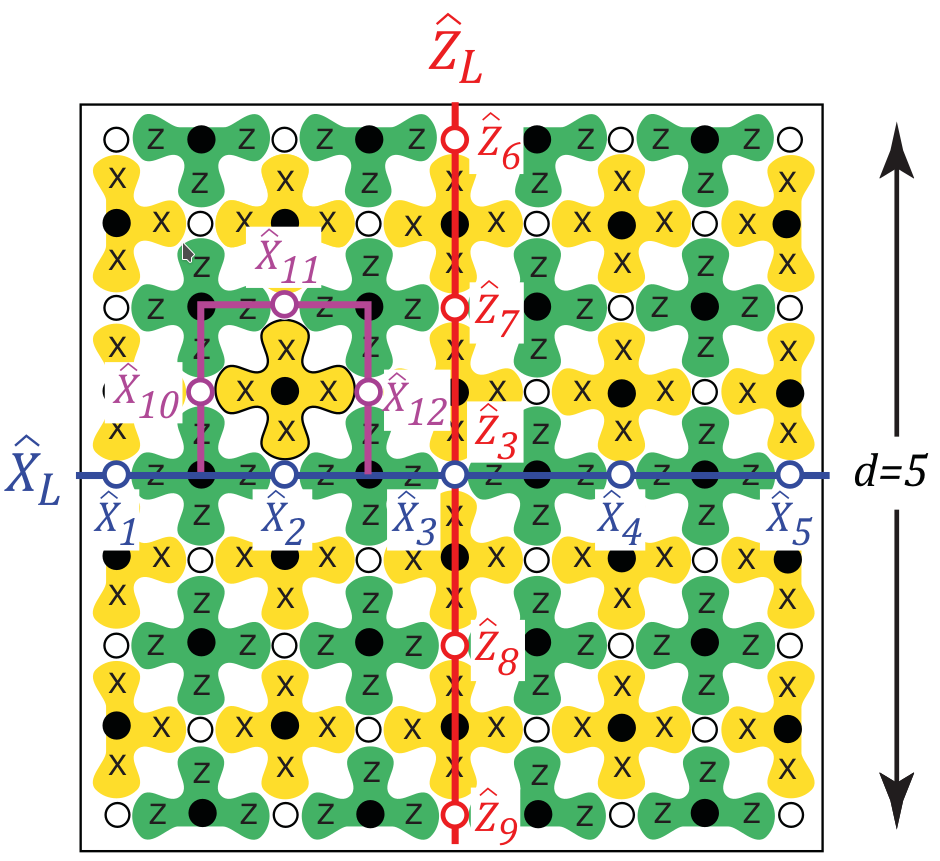
\includegraphics[width=0.4\textwidth]{images/surface_code.png}
  \caption{A 2D array of qubits representing a surface code of distance 5. Data
    qubits are white circles, each of which are connected to 2 $Z$- (green)
    and 2 $X$- (yellow) stabilizers respectively. The figure defines the logical
    operations $Z_L = Z_6Z_7Z_3Z_8Z_9$ (red) and $X_L = X_1X_2X_3X_4X_5$ (blue)
    that anti-commute. The purple line is a \texitit{stabilizer},
    $X_s = X_2 X_{10}X_{11} X_{12} $, an operation that does not affect the
    logical state of the qubit. Figure from \cite{fowler12_surfac_codes}.}
  \label{fig:surface_code}
\end{figure}

%measurement qubits or ancullary qubits?
Surface codes, a class of topological stabilizer codes, implement error
correction through a 2D array of qubits on a lattice, as shown in Fig.
\ref{fig:surface_code}. Computational states are stored in the \textit{data
  qubits} (white circles), whereas the \textit{ancillary qubits} (black circles)
perform parity measurements to check for errors. One of the advantages of
surface codes is that a QEC cycle only requires nearest neighbor interactions
which ``lowers'' the physical required connections among qubits greatly
reducing the ``cost to build them''. This, together with their planar
structure makes them a suitable choice when compared with other QEC codes (for
instance, Kitaev's toric code \cite{Kitaev_2003} or Steane's 7-qubit code
\cite{Steane_1996_QEC}). Furthermore, they have a very high error threshold
(1\%) relative to many other schemes \cite{terhal15}.
% All these positive
% characteristics have ... It is not difficult to see why surface codes have
% attracted so much attention recently as the most viable path forward in
% fault-tolerant computing. %Talk about this last sentenc


%%% Local Variables:
%%% mode: latex
%%% TeX-master: "QEC_paper"
%%% End:
